\begin{figure}[H]
    \begin{center}
        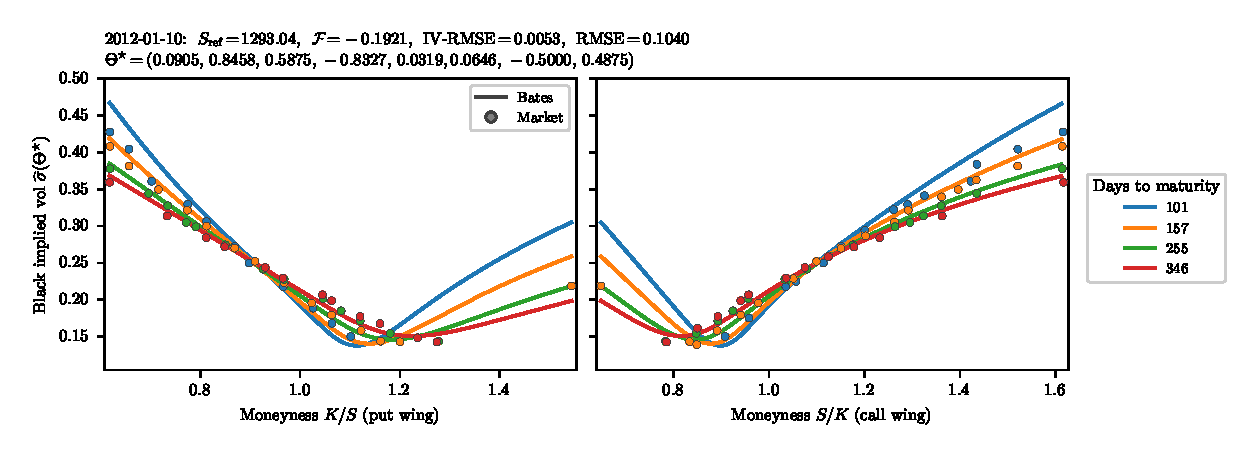
\includegraphics[width=\linewidth,keepaspectratio=false]{results/bates/smiles/figures/smiles_2012-01-10.eps}
        \captionsetup{font=tiny,skip=-2pt,belowskip=-2pt}
        \caption{Bates implied-volatility smiles for January 10, 2012: put wing (left, $K/S$) and call wing (right, $S/K$), with market trades scattered.}
        \label{Fig:smiles_2012-01-10}
    \end{center}
\end{figure}
\begin{figure}[H]
    \begin{center}
        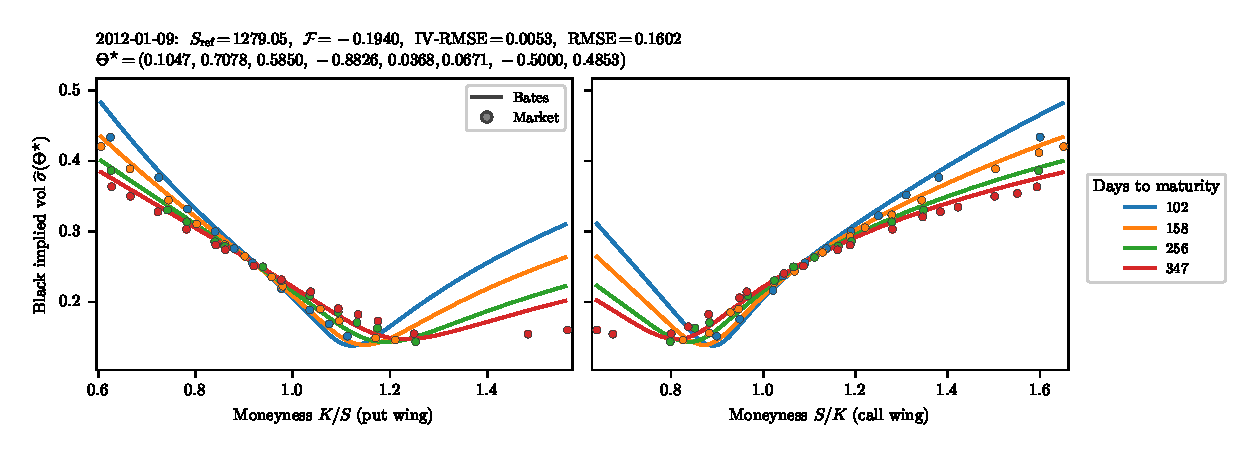
\includegraphics[width=\linewidth,keepaspectratio=false]{results/bates/smiles/figures/smiles_2012-01-09.eps}
        \captionsetup{font=tiny,skip=-2pt,belowskip=-2pt}
        \caption{Bates implied-volatility smiles for January 09, 2012: put wing (left, $K/S$) and call wing (right, $S/K$), with market trades scattered.}
        \label{Fig:smiles_2012-01-09}
    \end{center}
\end{figure}
\begin{figure}[H]
    \begin{center}
        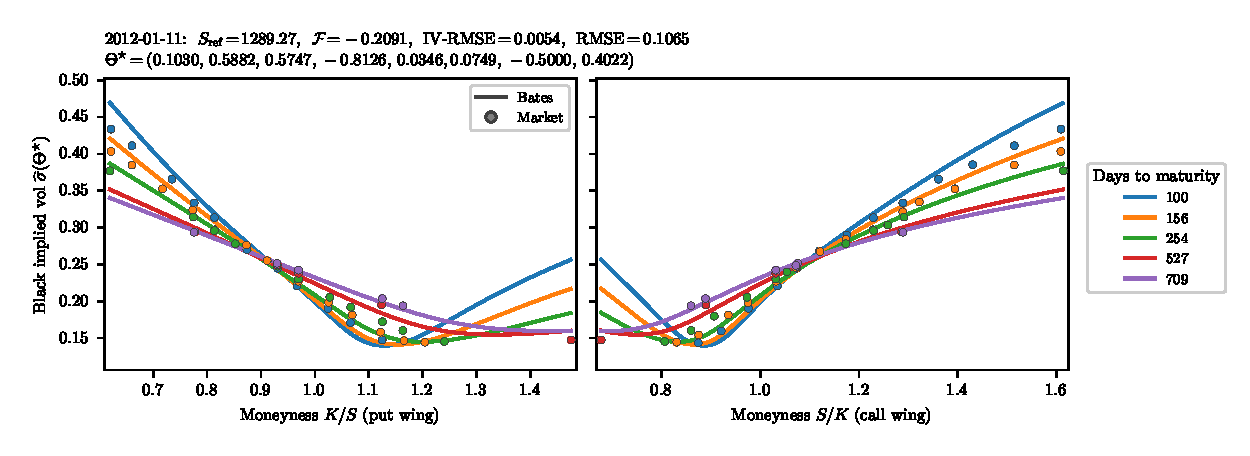
\includegraphics[width=\linewidth,keepaspectratio=false]{results/bates/smiles/figures/smiles_2012-01-11.eps}
        \captionsetup{font=tiny,skip=-2pt,belowskip=-2pt}
        \caption{Bates implied-volatility smiles for January 11, 2012: put wing (left, $K/S$) and call wing (right, $S/K$), with market trades scattered.}
        \label{Fig:smiles_2012-01-11}
    \end{center}
\end{figure}
\begin{figure}[H]
    \begin{center}
        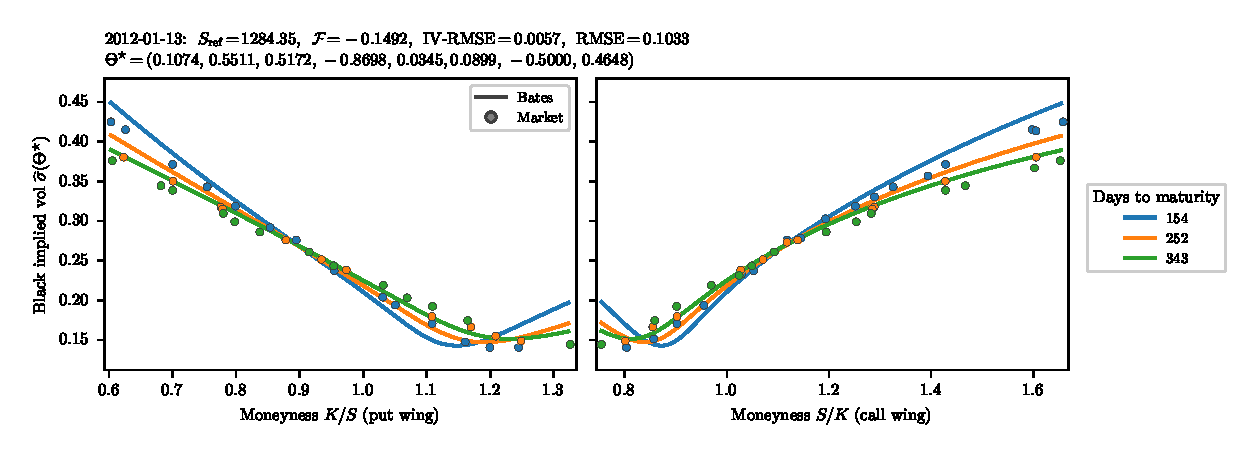
\includegraphics[width=\linewidth,keepaspectratio=false]{results/bates/smiles/figures/smiles_2012-01-13.eps}
        \captionsetup{font=tiny,skip=-2pt,belowskip=-2pt}
        \caption{Bates implied-volatility smiles for January 13, 2012: put wing (left, $K/S$) and call wing (right, $S/K$), with market trades scattered.}
        \label{Fig:smiles_2012-01-13}
    \end{center}
\end{figure}
\begin{figure}[H]
    \begin{center}
        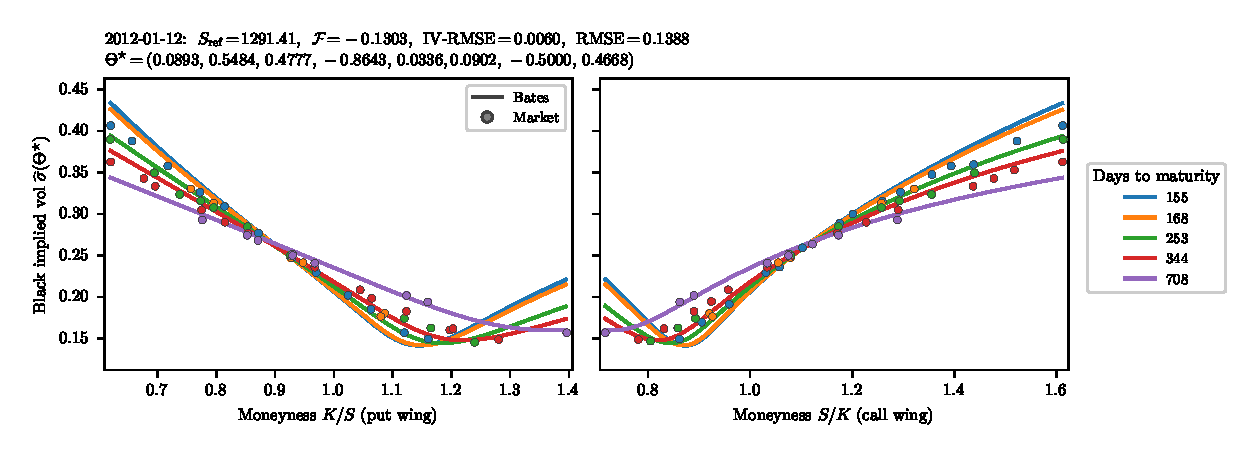
\includegraphics[width=\linewidth,keepaspectratio=false]{results/bates/smiles/figures/smiles_2012-01-12.eps}
        \captionsetup{font=tiny,skip=-2pt,belowskip=-2pt}
        \caption{Bates implied-volatility smiles for January 12, 2012: put wing (left, $K/S$) and call wing (right, $S/K$), with market trades scattered.}
        \label{Fig:smiles_2012-01-12}
    \end{center}
\end{figure}
\begin{figure}[H]
    \begin{center}
        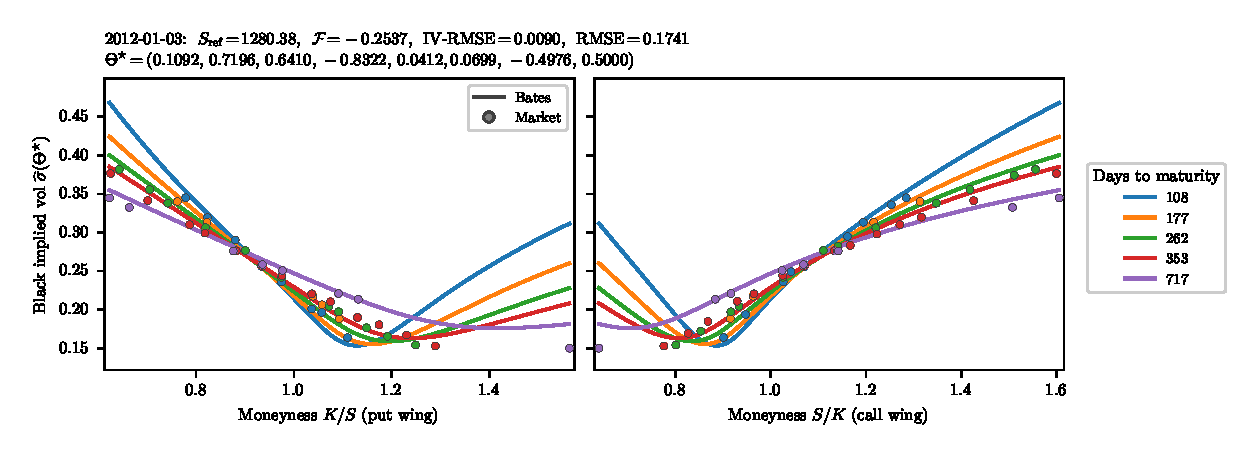
\includegraphics[width=\linewidth,keepaspectratio=false]{results/bates/smiles/figures/smiles_2012-01-03.eps}
        \captionsetup{font=tiny,skip=-2pt,belowskip=-2pt}
        \caption{Bates implied-volatility smiles for January 03, 2012: put wing (left, $K/S$) and call wing (right, $S/K$), with market trades scattered.}
        \label{Fig:smiles_2012-01-03}
    \end{center}
\end{figure}
\begin{figure}[H]
    \begin{center}
        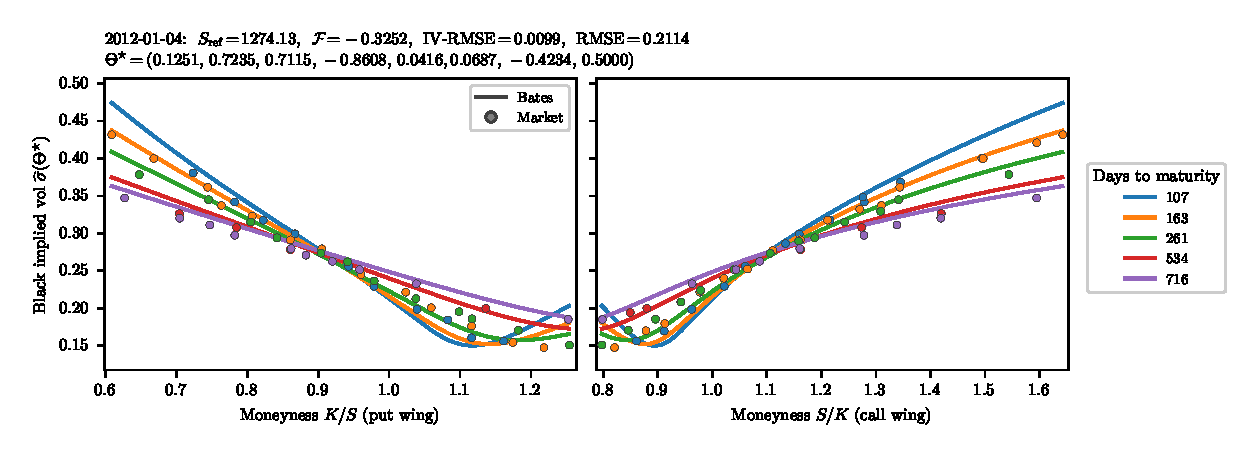
\includegraphics[width=\linewidth,keepaspectratio=false]{results/bates/smiles/figures/smiles_2012-01-04.eps}
        \captionsetup{font=tiny,skip=-2pt,belowskip=-2pt}
        \caption{Bates implied-volatility smiles for January 04, 2012: put wing (left, $K/S$) and call wing (right, $S/K$), with market trades scattered.}
        \label{Fig:smiles_2012-01-04}
    \end{center}
\end{figure}
\begin{figure}[H]
    \begin{center}
        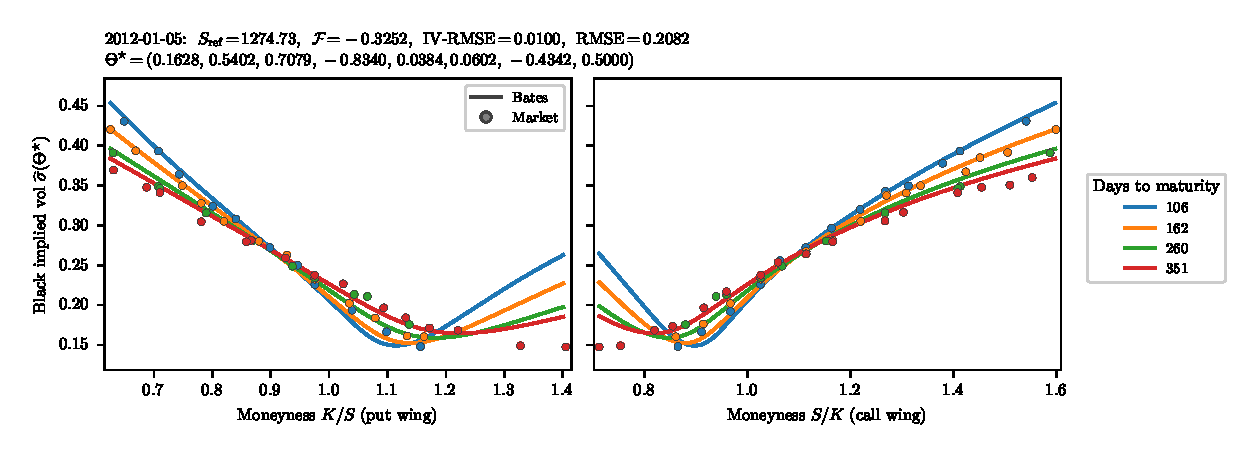
\includegraphics[width=\linewidth,keepaspectratio=false]{results/bates/smiles/figures/smiles_2012-01-05.eps}
        \captionsetup{font=tiny,skip=-2pt,belowskip=-2pt}
        \caption{Bates implied-volatility smiles for January 05, 2012: put wing (left, $K/S$) and call wing (right, $S/K$), with market trades scattered.}
        \label{Fig:smiles_2012-01-05}
    \end{center}
\end{figure}
